% !TEX root = ../SCXMLREF.tex


\subsection{Intrusion Detection System}
\label{sec:secbot}


The simple intrusion detection system is designed using an Application-Specific Integrated Circuit (ASIC) which connects to a buzzer and a sensor over a Serial Peripheral Interface (SPI) bus. The system is controlled via the ASIC on the SPI bus. At power-up, the ASIC sends commands over the SPI bus to initialize the sensor and the buzzer. After waiting for 50 milliseconds the ASIC enters its main routine, which makes the buzzer respond to the sensor. The statechart model of this system is limited to the ASIC and captures the initialization of the peripherals and the 50 ms wait. In the interest of simplicity we elide the details of the main routine.

The ASIC starts by initializing the buzzer. This involves sending a message over the SPI bus, and at the highest level of abstract we can additional implementation details. Once the message is sent (which will be indicated by some event saying that the SPI system is done), the ASIC moves on to initializing the sensor. After the ASIC moves into a waiting state for 50 ms, and finally moves into the state which represents normal operation.

A subsequent level of refinement adds a parallel state representing the SPI subsystem. The SPI subsystem is usually on an \textbf{Idle} state until the \textbf{send\_message} event occurs, at which point the SPI subsystem enters a state \textbf{Sending Message}, which represents sending the message, byte by byte. When the last byte of the message is sent, it raises the \textbf{spi\_done} event, allowing the other parallel state to continue, while SPI subsystem returns to idle.

The model can be farther refined by incorporating more details on how the initialization states, the wait state, and the SPI subsystem operate, including how they interact with each other. The \textbf{Initialize Buzzer} state constructs the SPI message to send, then it raises the \textbf{send\_message} event, and then it waits.
After \textbf{send\_message} is raised, the SPI subsystem reacts. It spins for a while in the \textbf{send\_byte} state, looping as many times as it takes to get to the last byte in the message. When the last byte in the message is sent, it goes back to idle and raises an event which allows the state machine on the left to proceed. The sensor is then initialized in a very similar manner to the buzzer. After both peripherals are initialized, the state machine goes into the \textbf{Wait 50 ms} state, where it  increments a counter until it reaches some maximum, then exits.



\begin{figure*}[t!]
    \begin{centering}
	    \begin{subfigure}[t]{0.5\textwidth}
	        \begin{centering}
	        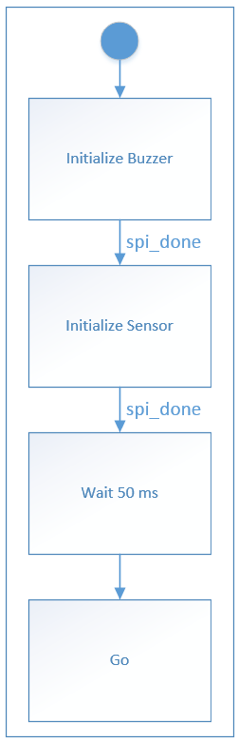
\includegraphics[height=3in]{figures/Buzzer}
	        \caption{Buzzer component high level abstraction}
	        \label{fig:Buzzer}
	        \end{centering}
	    \end{subfigure}

	    \begin{subfigure}[t]{0.5\textwidth}
	        \begin{centering}
	        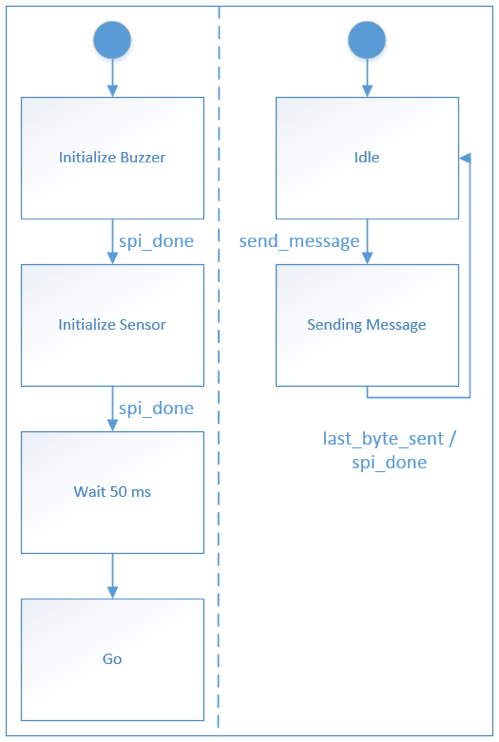
\includegraphics[height=3in]{figures/Buzzer&Sensor_1}
	        \caption{Statechart diagram for SecBot intrusion detection system}
	        \label{fig:BuzzerSensor_1}
	        \end{centering}
	    \end{subfigure}
	    \caption{First refinement including an abstraction of the sensor component}
    \end{centering}
\end{figure*}

\begin{figure}[]
  \begin{centering}
  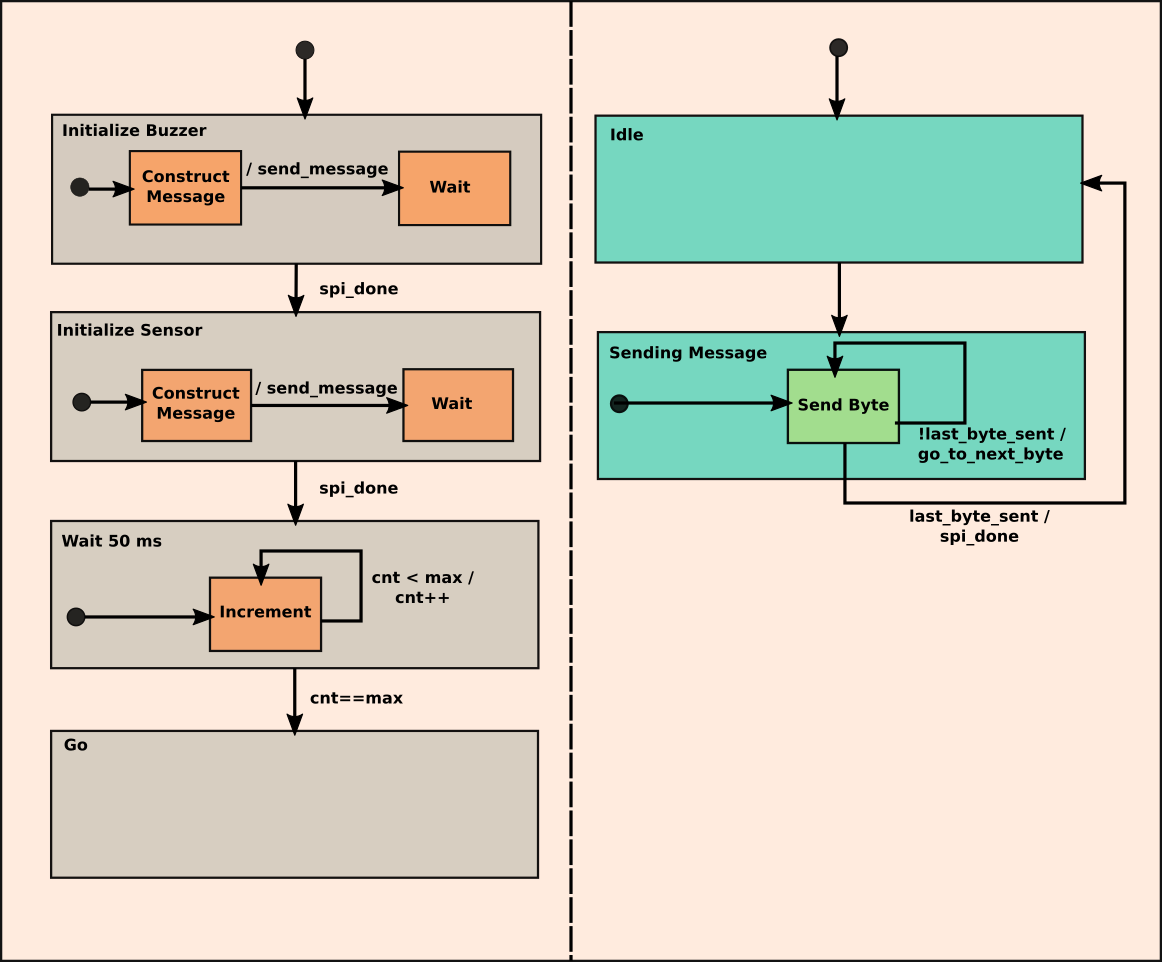
\includegraphics[width=0.8\textwidth]{figures/Buzzer&Sensor_2}
  \caption{Statechart diagram for SecBot intrusion detection system}
  \label{fig:BuzzerSensor_2}
  \end{centering}
\end{figure} 


\ColinCommented{introduce the secbot example showing how we would like to develop it in refinements}


